\section{Implementation}\label{Sec_Imp}

\subsection{Communication}
The already existing software is overwritten on the  built-in micro-controller of the WeMos Wifi Module which was developed to have a continuous listening to all the data  sent from the RFID reader even in case of no tags within the range. The good and bad RFID data readings are as seen in the fig.\ref{rfid_wifi}.\\
\begin{figure}[!htbp]
	\centering
	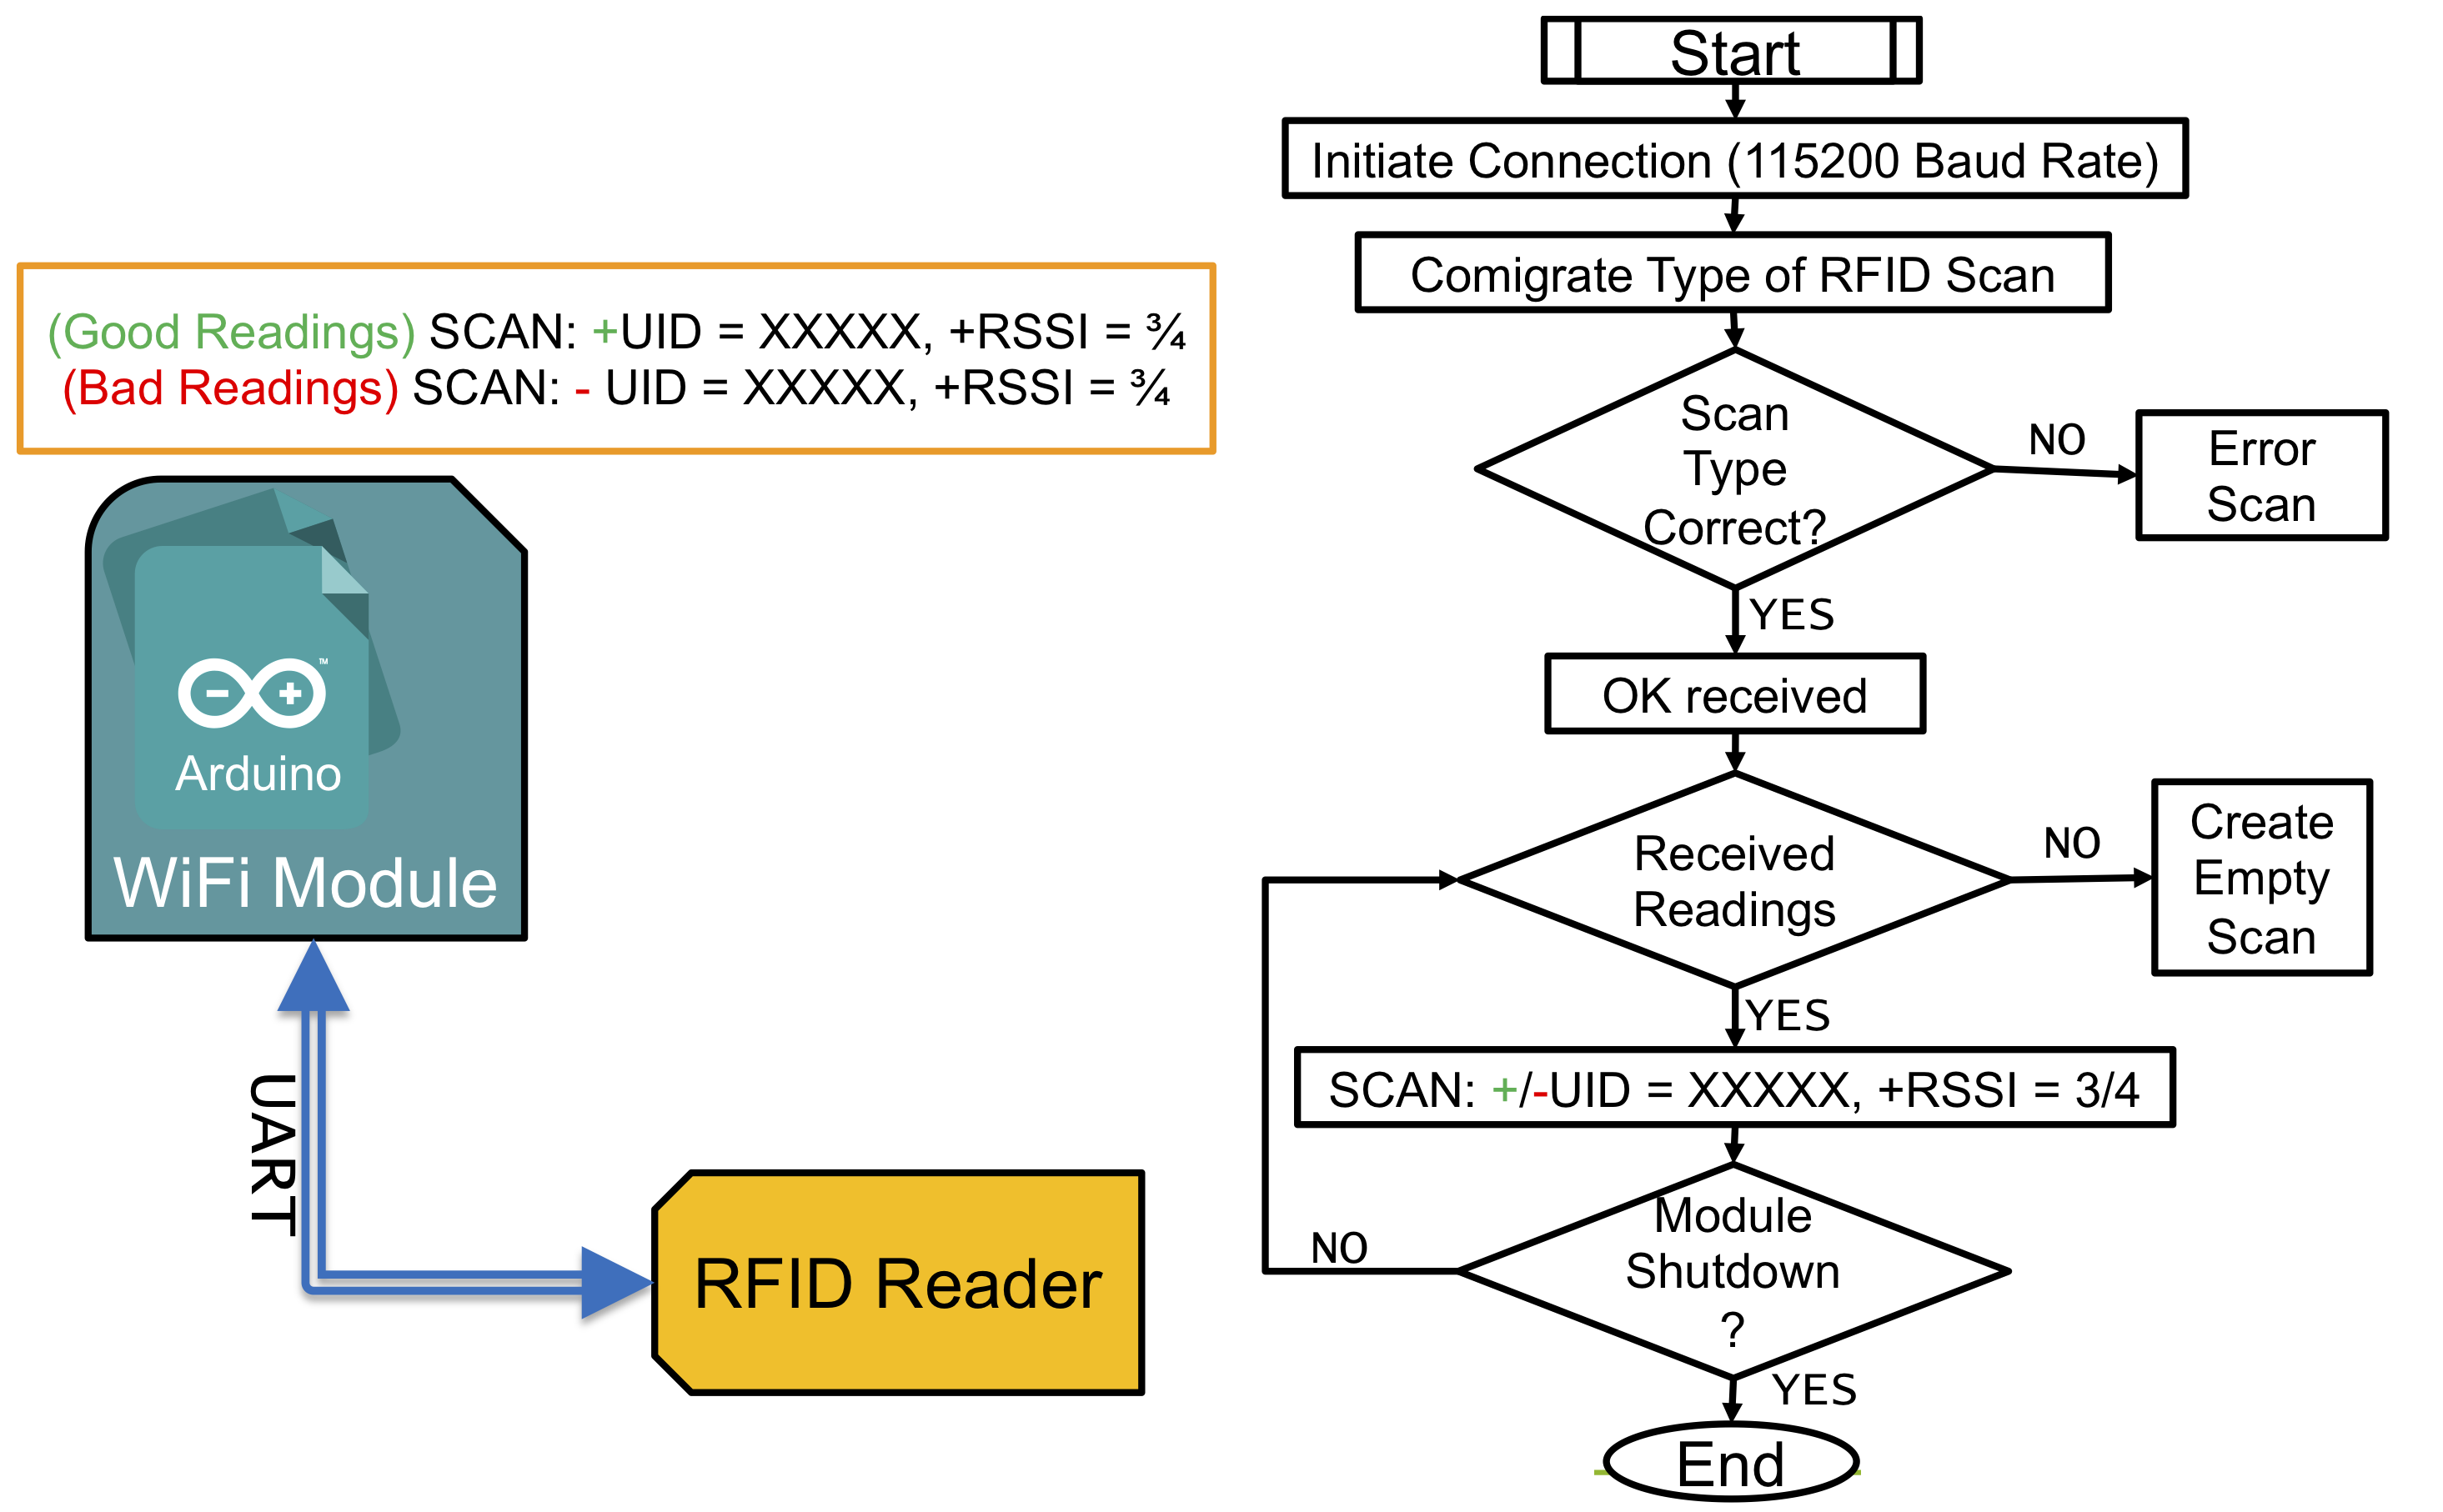
\includegraphics[width = 14cm]{Pictures/rfidwifi}
	\caption{RFID-WeMos Module Communication}
	\label{rfid_wifi}
\end{figure}\\
A TCP-IP communication is established within the network on the WeMos WiFi Module that start publishing the data which has been received from the reader. This communication is killed if and only if in the case of robot shutdown as shown in fig.\ref{wifi_network}.\\
\begin{figure}[!htbp]
	\centering
	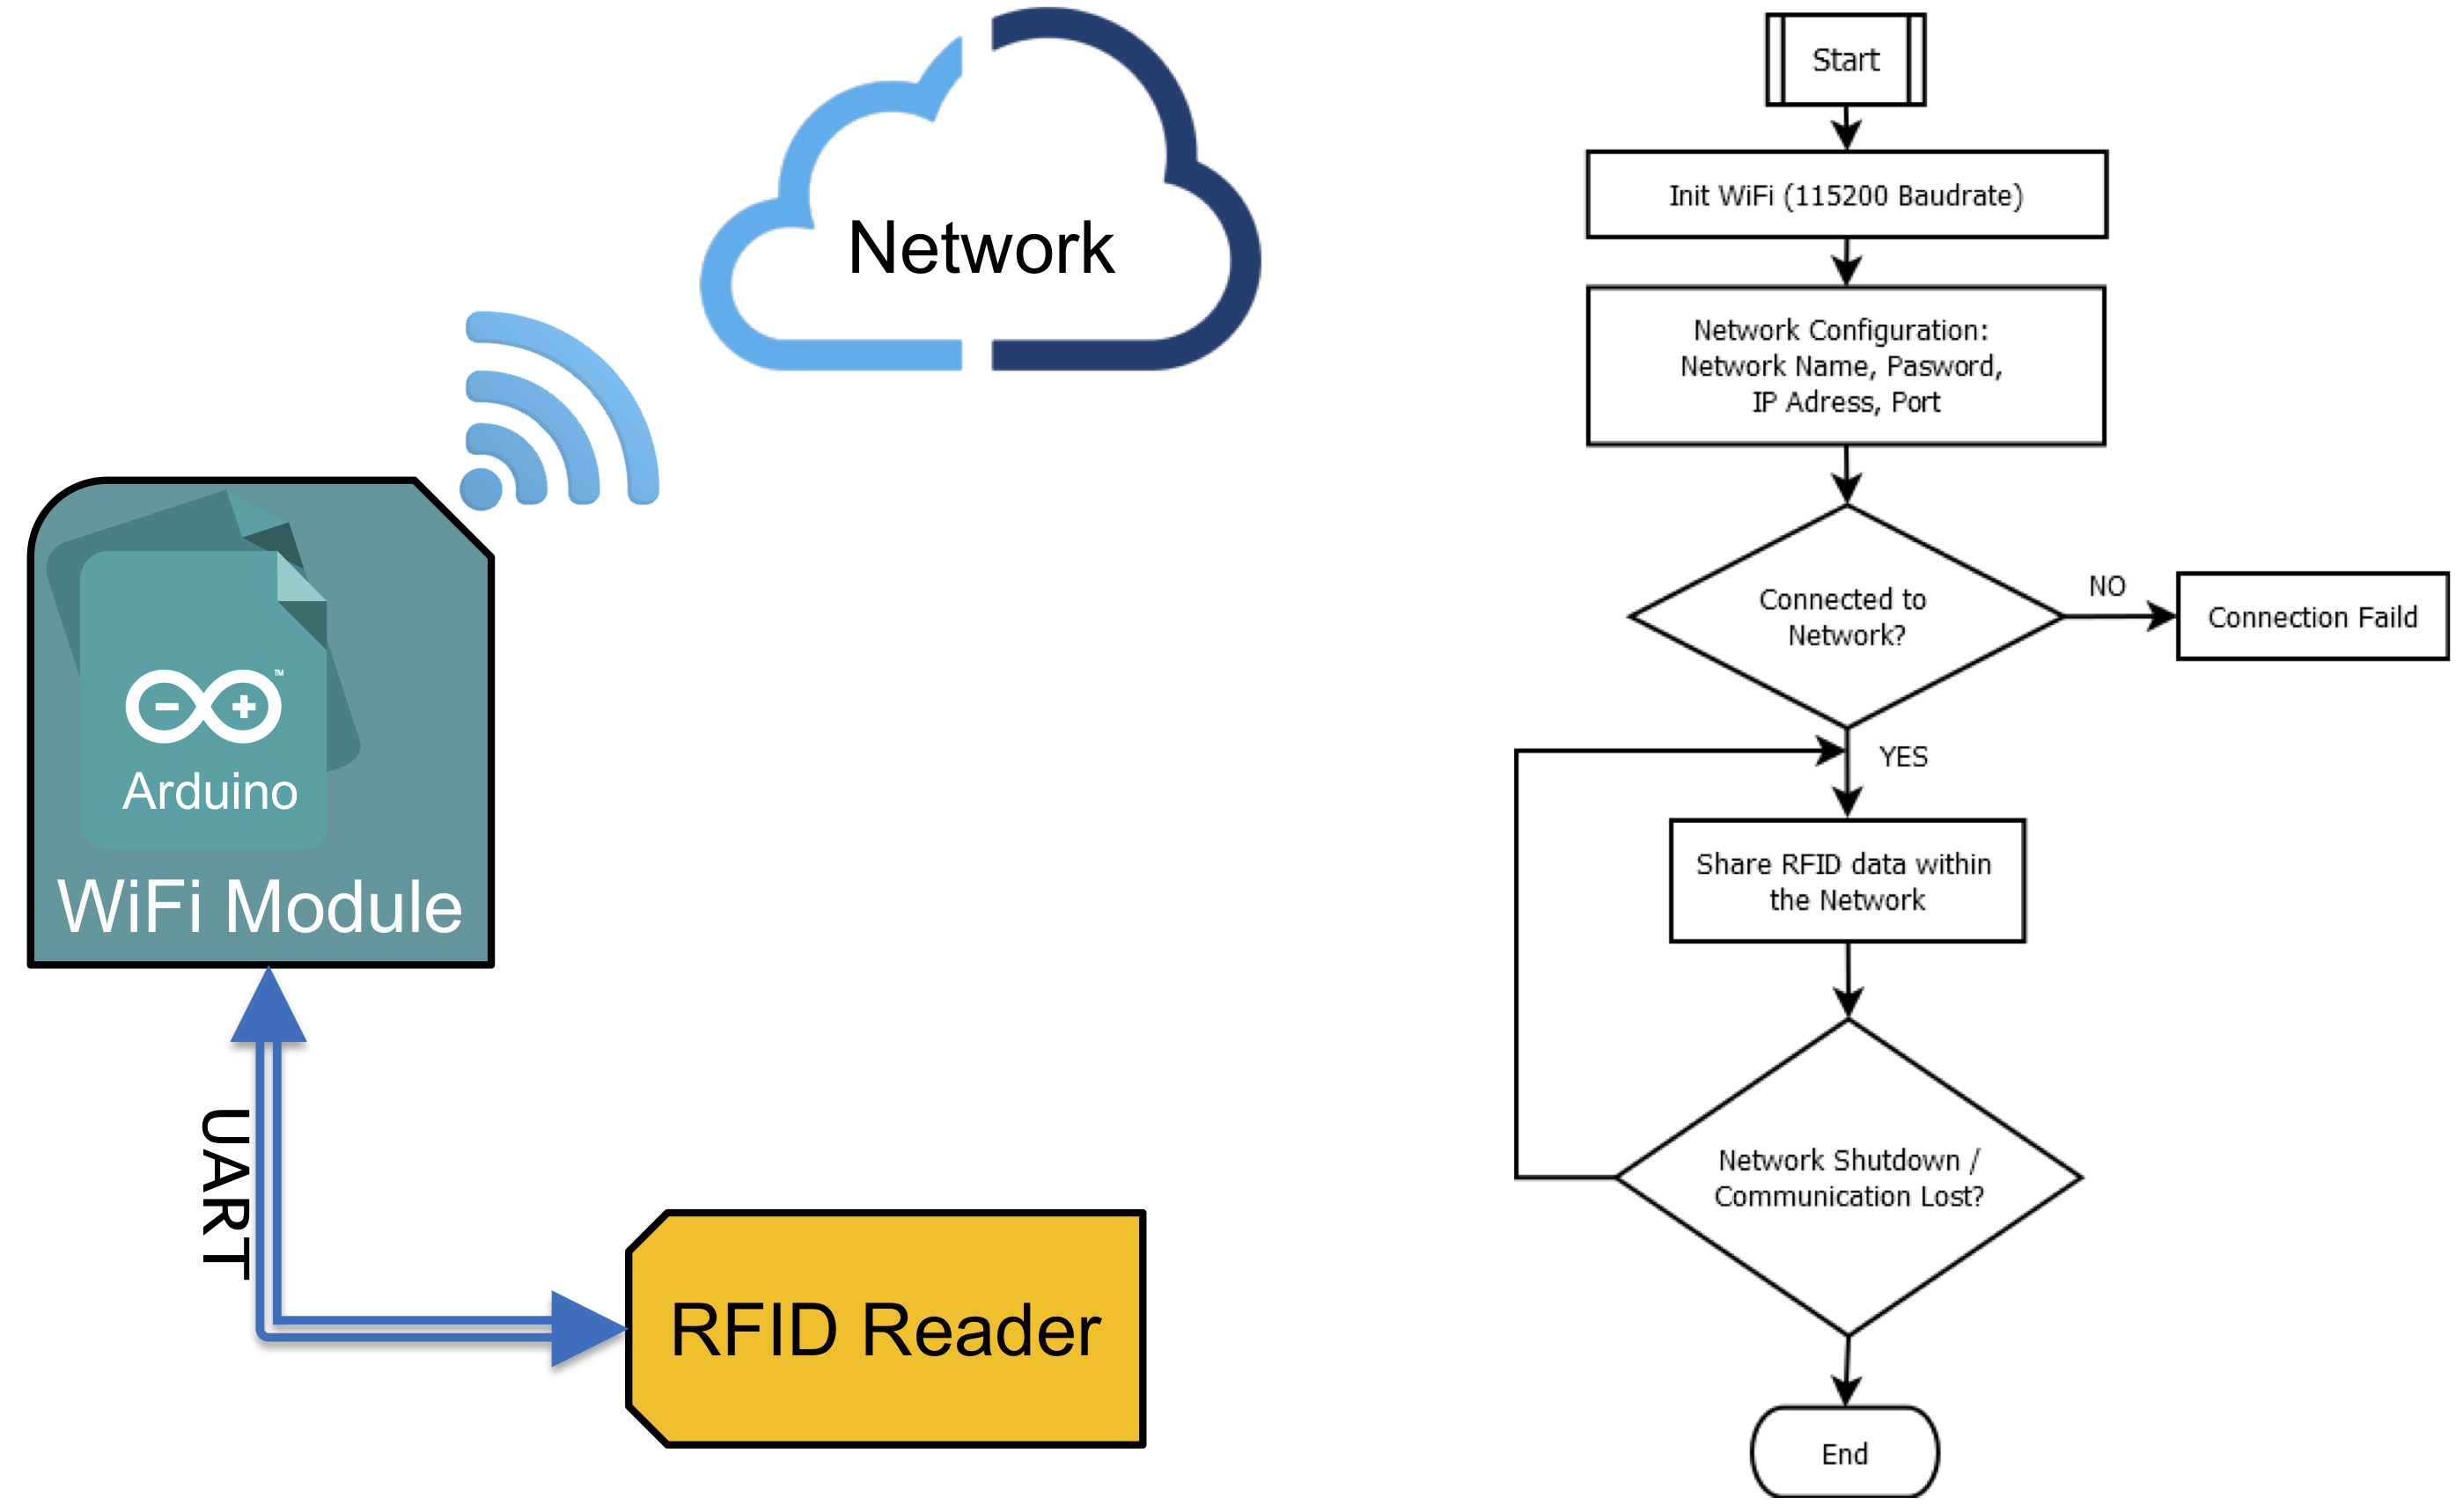
\includegraphics[width = 14cm]{Pictures/wifinetwork}
	\caption{WeMos Module Network Communication}
	\label{wifi_network}
\end{figure}
While on the other side on computer GUI (Graphical User Interface), the same type of communication is established (which should be in same network), and should grasp all the data that has been published by the WeMos WiFi module even if it no data is sent. This communication can be stopped from the GUI if needed as shown in fig.\ref{wifi_pc}.\\
\begin{figure}[!htbp]
	\centering
	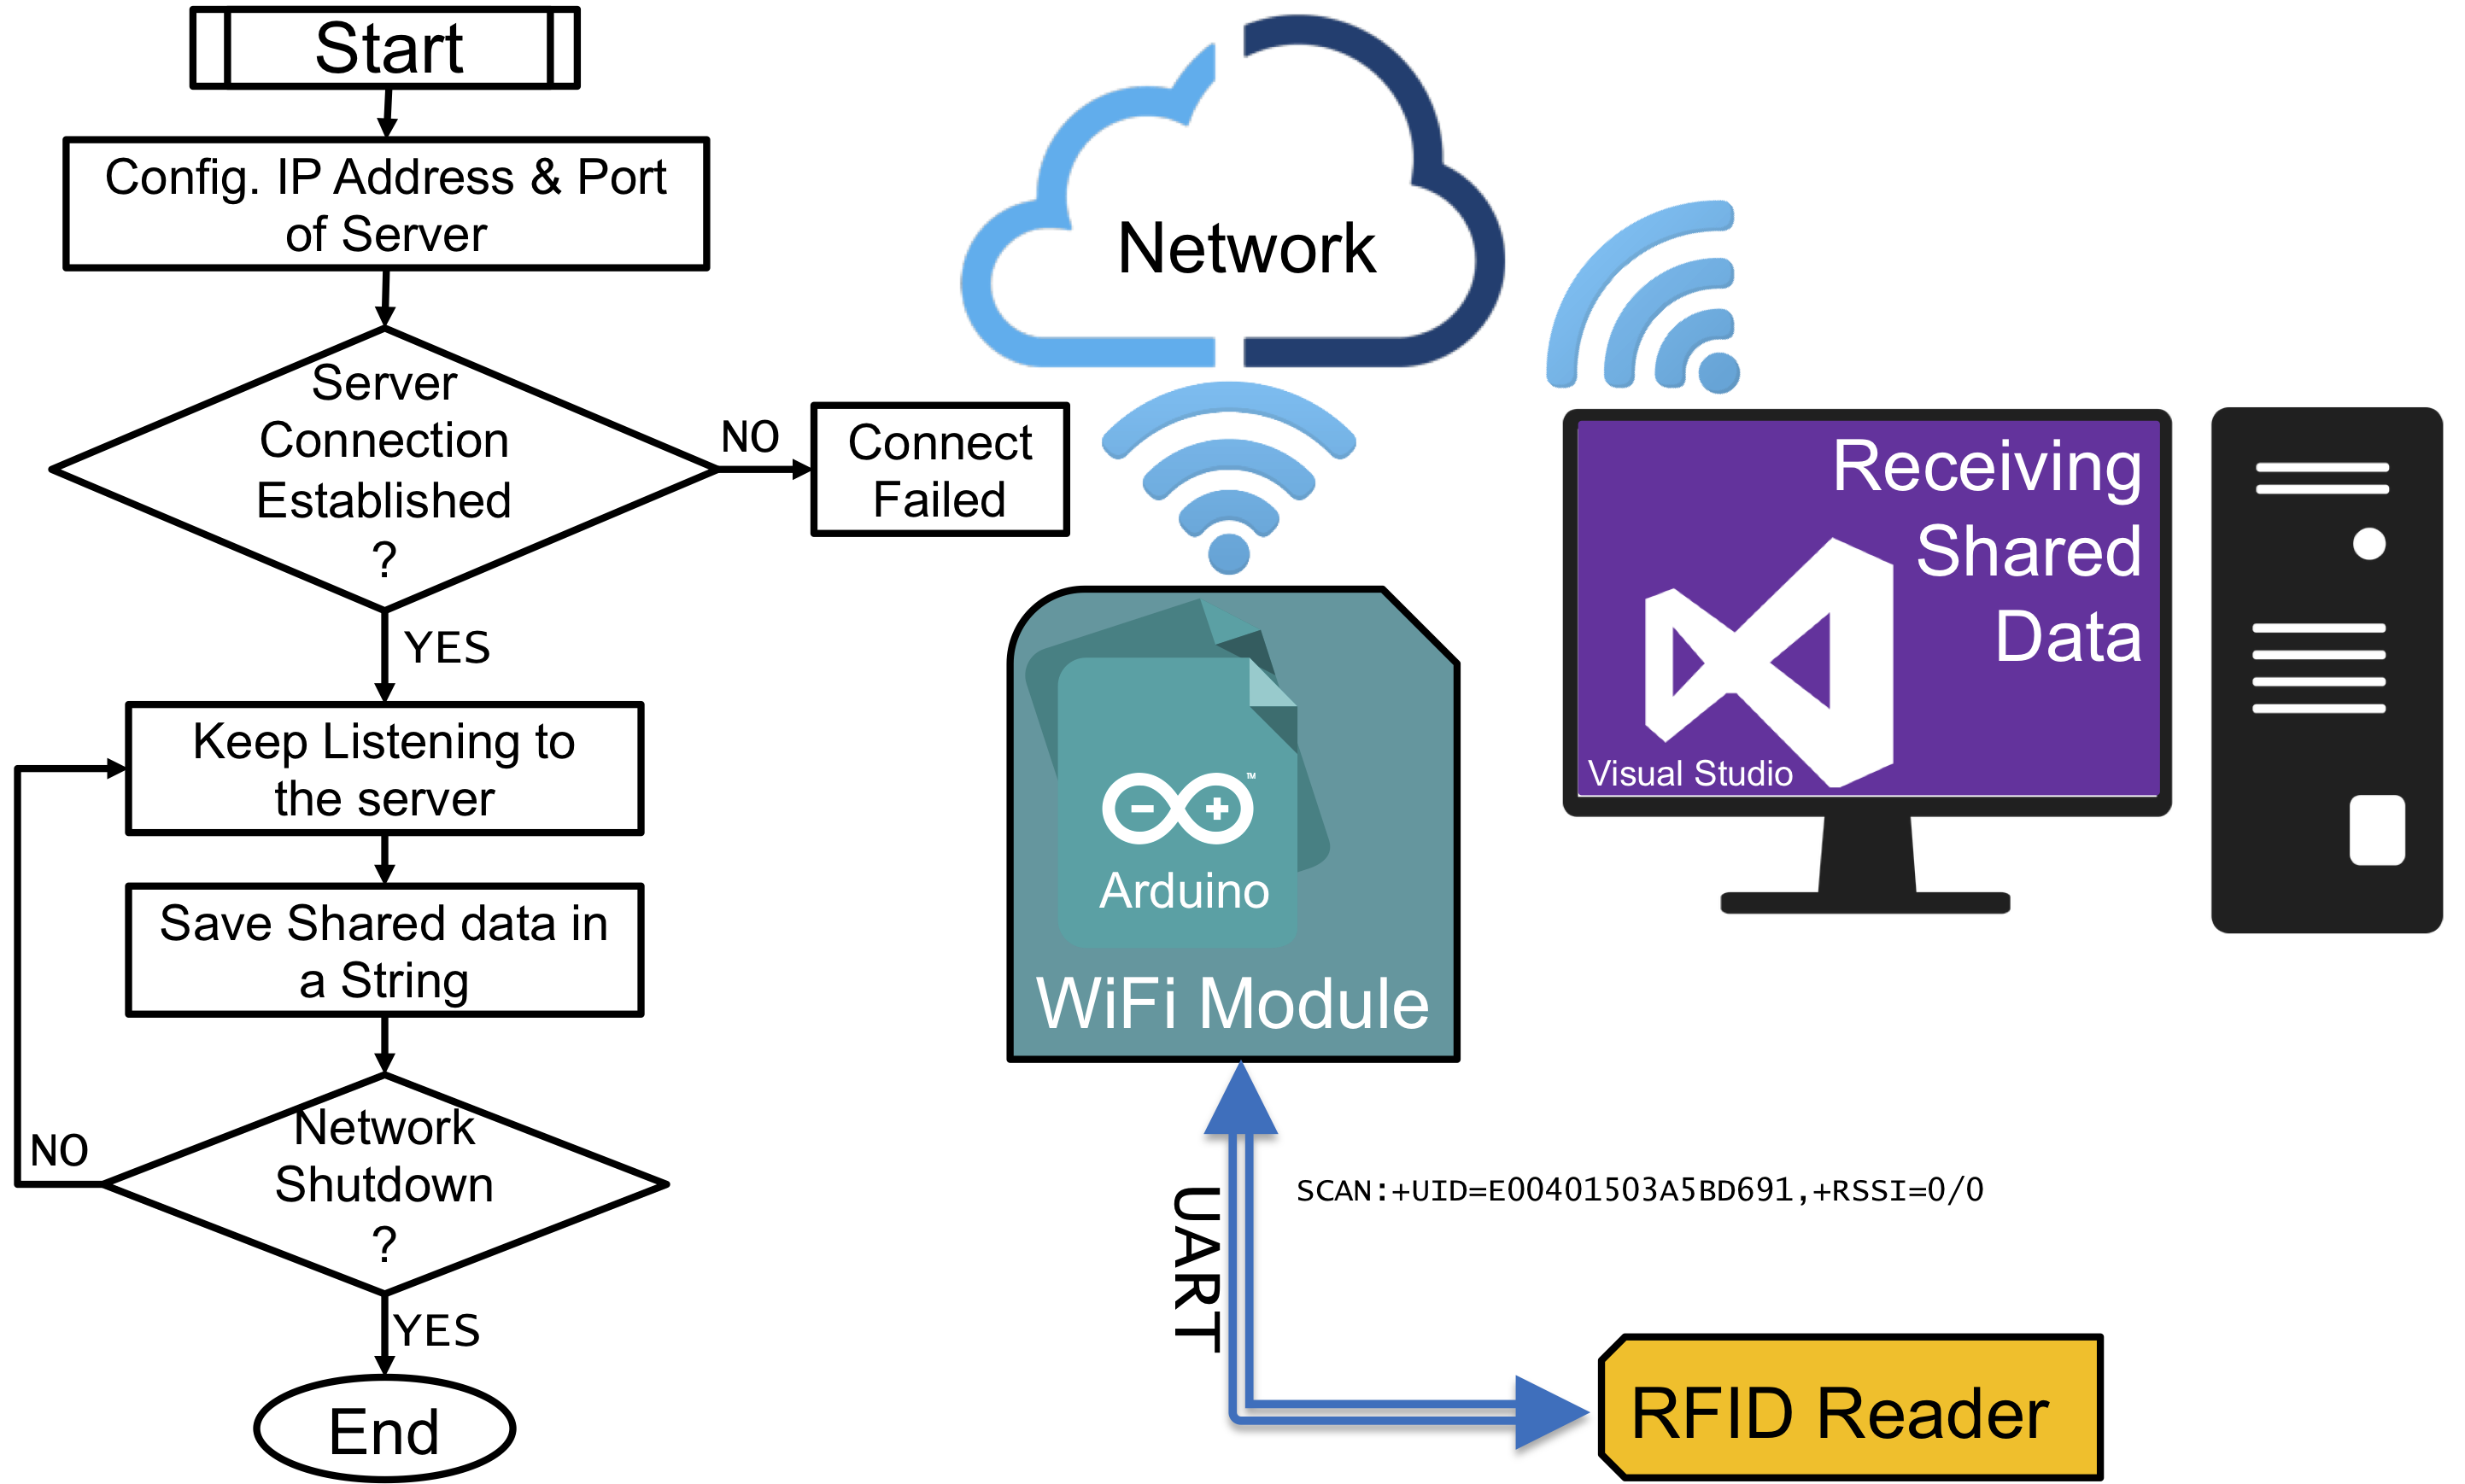
\includegraphics[width = 14cm]{Pictures/wifipc}
	\caption{Computer Network Communication}
	\label{wifi_pc}
\end{figure}\\
\subsection{Initialization procedure}
In the start-up phase, before running the pipeless plant with its AGVs the correct position and orientation of each and every vehicle are not known. Even though the controller is able to compute the position of the AGVs antenna in each point of time (t=0 included),  several AGV positions in the plants operation space can be discribed by one single antenna position. In fig. \ref{possible_initial_positions} four possible AGV positions with one common antenna position are pointed out. \\
\begin{figure}[!htbp]
\centering
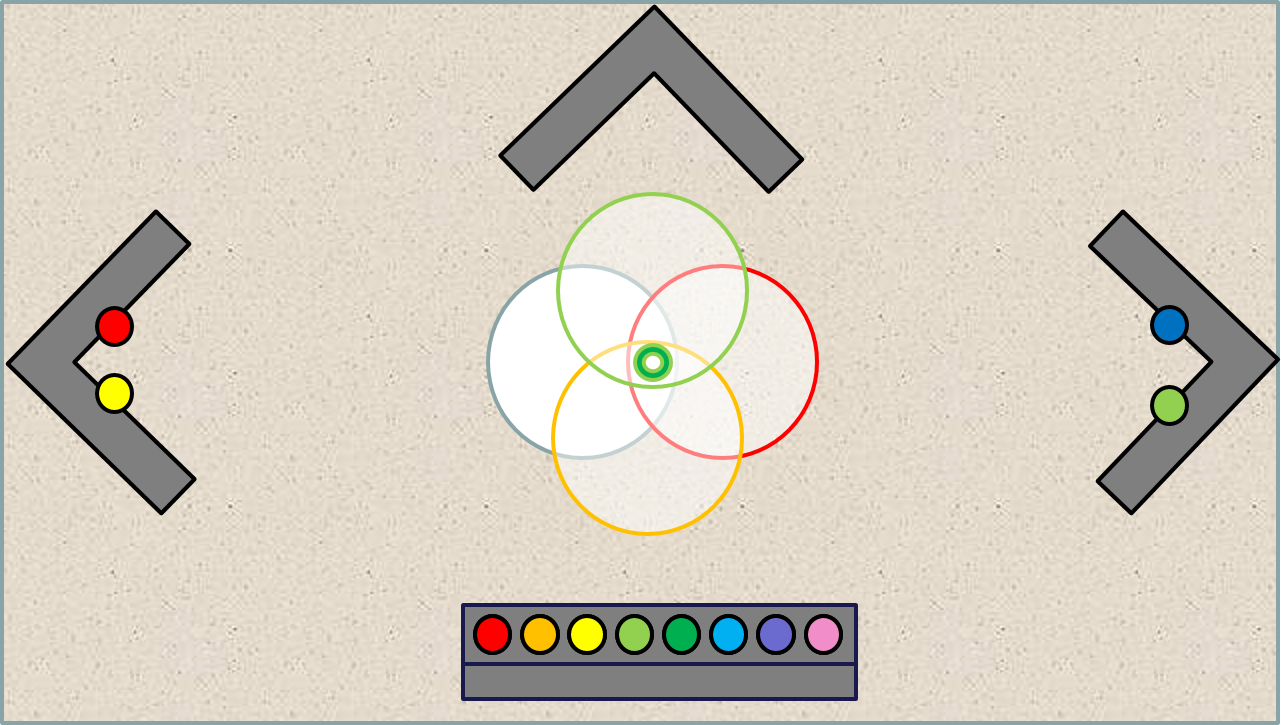
\includegraphics[width = 16cm]{Pictures/possible_initial_positions}
\caption{Different possible positions for one antenna position}
\label{possible_initial_positions}
\end{figure}\\
Since the position information is crucial for the plant, a procedure was set up to determine the starting positions of each and every AGV.
According to the fact, that the position and orientation of a single AGV is unknown at the beginning, some potential are taken into account. For instance, the plant contains several obstacles like the mixing stations, vessel storage, charging stations, plant edges and even other vehicles as represented in fig. \ref{hazards}.\pagebreak
\begin{figure}[!htbp]
\centering
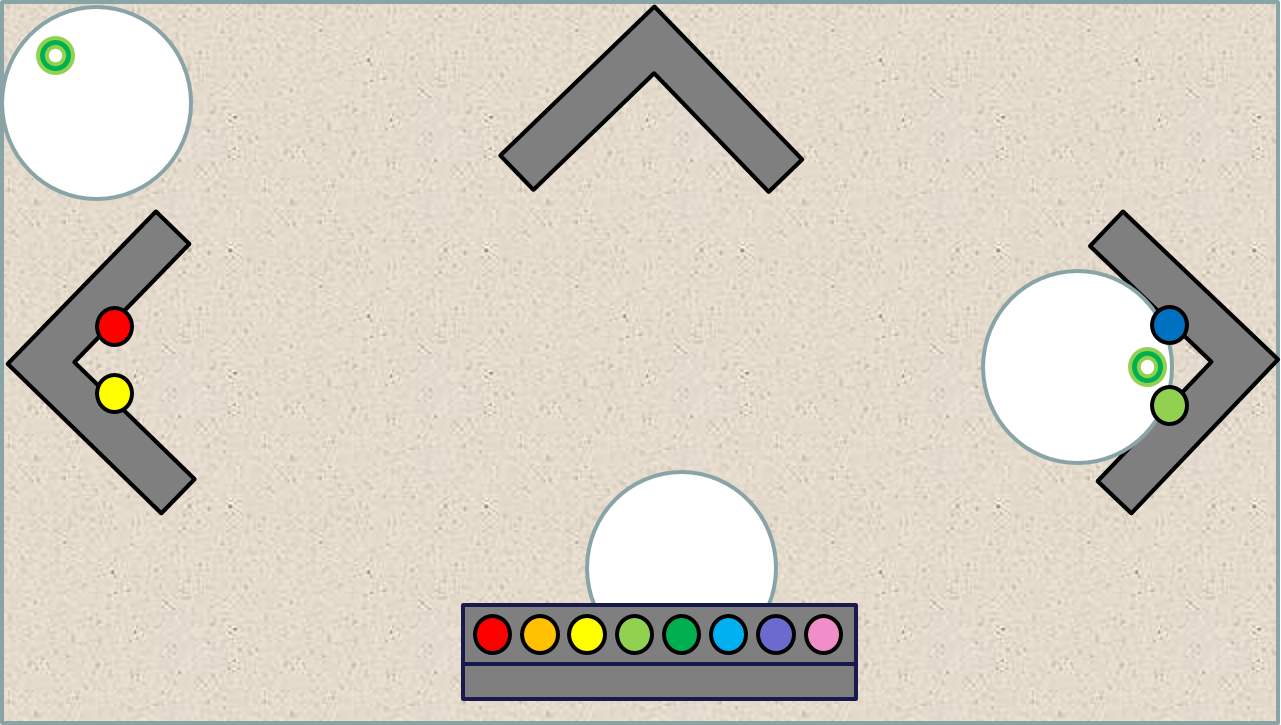
\includegraphics[width = 16cm]{Pictures/hazards}
\caption{Possible hazards/obstacles}
\label{hazards}
\end{figure}\\
With respect to these potential hazards collisions during the initialization procedure have to be avoided. This is realized by taking advantage out of the AGVs ability to turn around its z axis without a change of the AGVs center point in x and y direction. This ability of the AGV leads the way that each and every robot performs an initialization turn of 360$^\circ$ in which measurements are taken every 45$^\circ$ to estimate the specific positions and orientations of the AGVs. Furthermore, the decision process of the antenna position under the robot is dominated by the fact that the position of the center point does not change during a turn around its z axis. 
During the 360$^\circ$ turn the intervals in which the measurments have to be taken need to be known by the controller. The determination of these measurement points can be computed in two different ways. On the one hand the encoders of the AGV-wheels can be used to estimate the performed rotation. On the other hand, the time of a complete turn can be measured and used as a parameter in the procedure. In terms of simplicity the second option is used in the initialization procedure.  
Fig. \ref{SFC_Init_Procedure} illustrates a sequential flow chart which describes the movement and data processing during the initialization procedure.\\ 
\begin{figure}[!htbp]
\centering
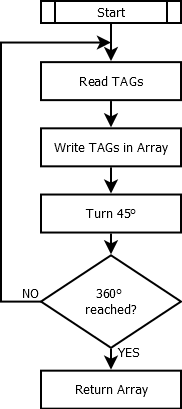
\includegraphics[width = 4cm]{Pictures/SFC_Init_Procedure}
\caption{Flow Chart: Initial procedure 360$^\circ$ turn}
\label{SFC_Init_Procedure}
\end{figure}\\\\\\\\\\\\\\\\
The initialization procedure for AGV No. 1 is created and can be started in the GUI in the test environment. In the first place an integer number is given to the field called Sleeptime. This integer number is interpretated in milliseconds and describes the time of rotation. Even though a time for a complete turn of 45$^\circ$  has been found at around 1125ms it has to be said that this time strongly depends on the battery charge of the AGV. After the desired turning time is given to the GUI the initialization is started by pushing the button Initialization, located over the input box in fig.  \ref{Screenshot_Test_environment}.\\
\begin{figure}[!htbp]
\centering
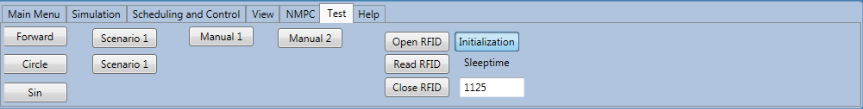
\includegraphics[width = 16cm]{Pictures/Screenshot_Test_environment}
\caption{Test environment in GUI}
\label{Screenshot_Test_environment}
\end{figure}\\
In the second step, after the procedure was started, all the available IDs and their respective RSSI in the current reading range of the RFID-Reader are read. The reading is performed in the Automatic Scan mode of the RFID reader\cite{KTSSysteme.2017}. With the included timestamp for every measurement a delay of minimum 30ms between each tag information was detected. With respect to this delay the antenna has to stop a specific period of time at each measuring point to deliver correct data of all the reachable tags. Experiences have shown, that a measuring time between one and two seconds delivers the best results. During this time every 100 ms new measurment information are taken. In order to save the single TAG information of each and every measuring point an initially empty array with 14 columns and 8 rows is created. 
The number of rows is derived by the fact that measurements are taken at every 45\textdegree. \\
\begin{align}
Rows = 360^\circ/45^\circ = 8\\
\end{align}
The first seven columns in the array are filled by the received TAG IDs and the last seven entries are filed by the respective RSSI. \\
The number of columns is derived by the fact that at each and every measurement point in the used test environment, information of maximal seven TAGs can be read. \\
\begin{align}
Columns = max. no. of  tags * 2 = 7 * 2 = 14\\
\end{align}
Once the received data is saved in its corresponding row, the AGV turns around 45\textdegree  to place the antenna at the next measuring point. An AGV turn is realized by setting the velocity of the right and left wheel in different directions. During the turning sections the velocity is set to 100 mm/s or rather -100 mm/s. 
This procedure of reading information, writing information in the initialization array and turning 45$^\circ$  to the next measuring point is repeating itself until a 360$^\circ$  turn is performed. After a successful initialization turn the corresponding array of measurement information can look like the example in table \ref{Init_Array}.
\begin{table}[!htbp]
\centering
\begin{tabular}{|c|c|c|c|c|c|c|c|c|c|c|c|c|c|}
\hline
4&1&5&2&3&&&0&0&1&7&0&&  \\ \hline
5&3&&&&&&2&3&&&&&  \\ \hline
3&5&&&&&&2&2&&&&&  \\ \hline
9&8&6&5&&&&1&1&1&2&&&  \\ \hline
9&7&8&6&4&5&&2&0&6&0&0&2&  \\ \hline
4&7&5&8&&&&0&2&3&3&&&  \\ \hline
5&4&7&8&1&&&2&5&0&0&0&&  \\ \hline
2&4&1&5&&&&0&2&2&0&&&  \\ \hline
\end{tabular}
\caption{Filled array after 360$^\circ$ turn}
\label{Init_Array}
\end{table}\\

\subsubsection{Recording and filtering data}
To read the ID and RSSI of all the TAG laying in the reading range the RFID-reader is set to its Automatic mode and its Anticollision is switched on. In this mode packages of strings with a length of 35 characters are received by the plans computer. Even though these 36 character strings contain all the information of the TAG which is needed some effort has to be taken to seperate the useful parts which are processed in the localization algorithm.\\
With exception of the information each string contains, the structure itself is always the same. In the first five characters the substring ``\textit{SCAN:}'' is detected and deleted for the further process. The first important character is found in the sixth slot of the string. Here either a ``\textit{+}'' or a ``\textit{-}'' is written. With the help of this sixth slot it is distinglished wheather the current reading is complete or not. In order to guarantee the correctness of the received information the measurments are filtered by the ``\textit{+}'' and the measurments in which a ``\textit{-}'' is included are ignored in the further processes. After the indicator for complete and in complete readings a introduction to the ID is indicated by  ``\textit{UID=} '' and cut out of the string. The next 16 characters defines the unique identification of the specific TAG. As a last useless string, which has to be cut out, with the structure ``\textit{.RSSI=}'' is found directly after the ID. As a result the 16 character hexadecimal ID and its respective RSSI are seperated from the received string. Since the ordered tag IDs differ each other just in the last three numbers these numbers are transformed in a decimal number before UID and RSSI are used for further computations.\\
\begin{table}[!htbp]
\centering
\begin{tabular}{|l|l|}
\hline
\multicolumn{2}{|c|}{\textbf{String Transformation}}                               \\ \hline
\multicolumn{1}{|c|}{\textbf{Complete}} & \multicolumn{1}{c|}{\textbf{Incomplete}} \\ \hline
SCAN:+UID=E00401503A5BD691,+RSSI=0/0    & SCAN:-UID=E00401503A5BDAE4               \\ \hline
UID=E00401503A5BD691,+RSSI=0/0          &                                          \\ \hline
E00401503A5BD691 0/0                    &                                          \\ \hline
1681 0                                  &                                          \\ \hline
\end{tabular}
\caption{String preperation}
\label{string_prep}
\end{table}

\subsubsection[Analysing data]{Analysing data\footnote{Stefan}}
In the next step of the algorithm the previous described filled array is analyzed. To estimate the position and orientation of the AGV the array has to include two valid sets of each two valid measuring points.  During this analyzation the single measurement point-sets are validated in terms of following restrictions:\\\\
1.: At the two valid measurement point each contains at least three tags\\
2.: The other measurement point in one set needs to have a distance of 180$^\circ$  to the first.
\pagebreak\\
In terms to get the adequate sets of measurment points the array is analyzed row by row. The stepwise workflow is vizialized in fig. \ref{Analyze_Array}.\\
\begin{figure}[!htbp]
\centering
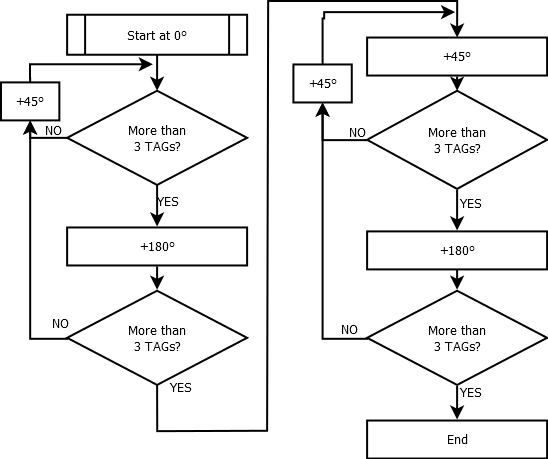
\includegraphics[width = 10cm]{Pictures/AnalyzeArray}
\caption{Flow Chart: Analizing measurment points}
\label{Analyze_Array}
\end{figure}\\
Initially the first row which represents the measurement at the point 0$^\circ$ is checked in terms of the number of readable tags. If this specific number is higher or equal three the transition is acknowledged as true and the same query will be performed at the measurement point with a distance of 180$^\circ$ to the former measurement point. If this next measurement point can be described as valid, the first valid set of two measurement points is found. If, on the other hand, the number of readable TAGs are less than three, which means that the triangulation algorithm cannot be performed, the current measurement point is ignored and the next measurement point is evaluated.
Each of this sets of two measurement points is saved as a 1x2 array called Solution 1 and Solution 2 is used for the estimation of the position of the measurement points which is explained in the section 7.2.4 Estimation of initial position and orientation.\\
%

\subsubsection[Selection of correct distance related to RSSI]{Selection of correct distance related to RSSI \footnote{Stephan}}
In a first step the multiple occurring data points (see tbl.\ref{RSSI_Dis_data}) are divided into three groups (max, middle and min) where max means the maximal possible distance related to one RSSI and so on.\\ 
The measurements have shown that it is not trivial to define the correct distance related to most of the RSSI. The involved algorithm selects the correct distance out of the multiple possible solutions and is shown in fig. \ref{BestID}:\\
\begin{figure}[!htbp]
\centering
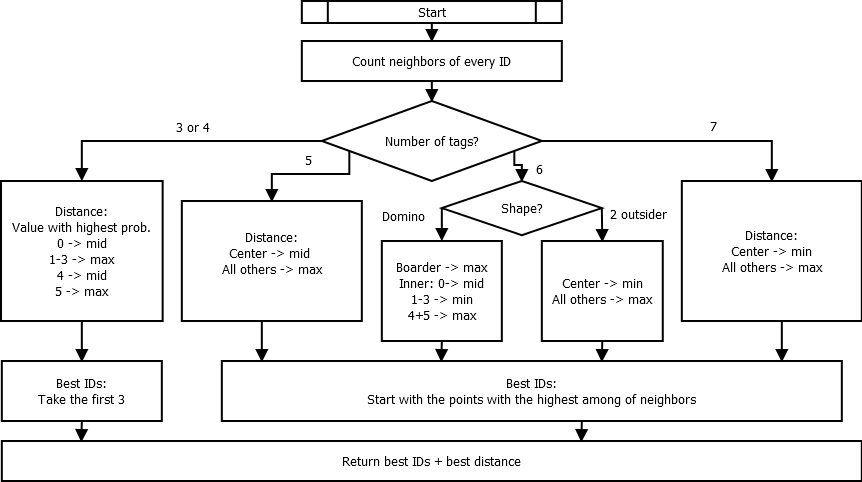
\includegraphics[width = 16cm]{Pictures/BestIDs}
\caption{Flow Chart: Selection of correct distance and most proper IDs}
\label{BestID}
\end{figure}\\
To distinguish between the multiple possible solution for one RSSI, the algorithm defines the shape of the pattern of tags based on the number of tags at each measurement and the number of the neighbours each tag has. At each measurement point in this scenario several numbers (4-7) of detected tags are possible. The different shapes can be found in the tbl. \ref{ID_shapes}.\\
\begin{table}[!htbp]
\centering
\begin{tabular}{|c|c|c|c|c|c|}
\hline
\begin{tabular}[c]{@{}c@{}}Number of \\ detected tags \end{tabular}  & 4 & 5 & 6 (Domino) & 6 (2 alone)& 7 \\ \hline
Unique shapes        & 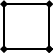
\includegraphics[width = 1.3cm]{Pictures/Shape1} & 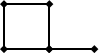
\includegraphics[width = 2.6cm]{Pictures/Shape2} &   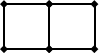
\includegraphics[width = 2.6cm]{Pictures/Shape3} & 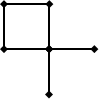
\includegraphics[width = 2.6cm]{Pictures/Shape4} & 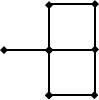
\includegraphics[width = 2.6cm]{Pictures/Shape5}\\ \hline
\end{tabular}
\caption{Possible shapes of pattern}
\label{ID_shapes}
\end{table}\\
Going back to the flow chart fig.\ref{BestID} the first step is to count the number of neighbours each tag has. With this information, the position of the tag in the pattern can be detected. For example, a tag with 3 neighbours in a pattern of 5 tags, is the center of this pattern.\\
After the number of tags at each measurement point and the position of each tag are defined, the selection of the correct distance will be performed based on the highest probability. To know the highest probabilities an analysis of measurements with emulated data has been done.\\
As an example 4 detected tags are leading to the fact that the position of the antenna should be very close to the center of this square. If in this case a RSSI of 4 is detected, the middle value (5.8 cm) will be taken. \\
Afterwards the most suitable three IDs will be selected, in case where more then three are detected. The algorithm takes at first the ID with the highest amount of neighbours, because these tags are close to the position of the antenna and have probably a value of 6 or 7 and are uniquely defined. In the case where several tags with the same number of neighbours, the first ID (number increasing) will be taken. \\
The return of the function is an array (2x3) with the indices of the chosen IDs and the correct distance. The correct distance will be indicated by the number 0,1 and 2. 0 means the maximal, 1 the middle and 2 the minimum possible value related to one RSSI. For example 
\[
\begin{bmatrix}
    3 & 2 & 4\\
    2 & 0 & 0 
\end{bmatrix} 
\]
leads to the choice of the maximal value of the RSSI of the fourth detected ID and the minimum value of the RSSI of the third and the fifth ID in the recorded array at this measurement point. \\

\subsubsection[Estimation of initial position and orientation]{Estimation of initial position and orientation \footnote{Stephan}}
As mentioned in chapter \ref{Sec_Imp_Ini}, the main idea to estimate the initial position is to find the intersection point, which lies in the middle of the measurement points.\\
To compute this position, the algorithm uses trilateration at every suitable measurement point to estimate its position. For trilatertion are three defined positions plus three radii necessary, which are available after the selection of the correct distance and proper IDs.\\
\begin{figure}[!htbp]
\centering
\begin{minipage}{.5\textwidth}
\centering
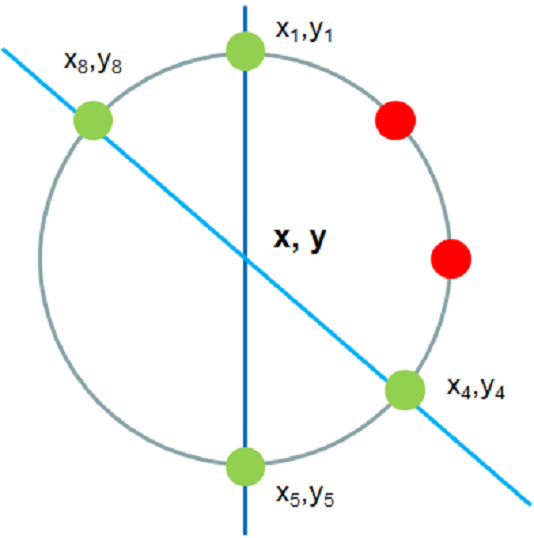
\includegraphics[width=5.5cm]{Pictures/Center_Rob} %
\caption{Computing the center of the robot}
\label{Center}
\end{minipage}%
\begin{minipage}{.5\textwidth}
\centering
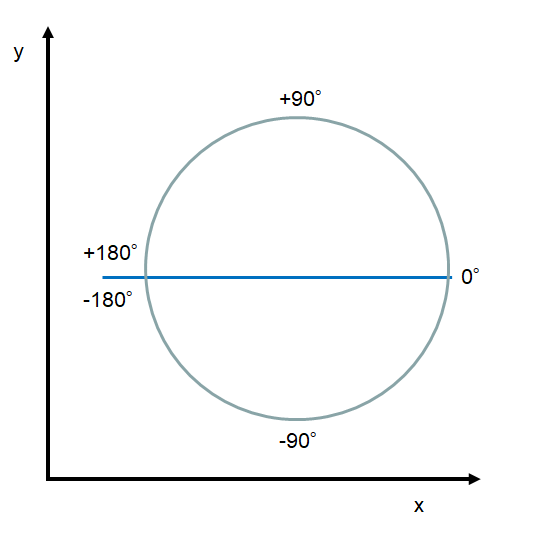
\includegraphics[width=5.5cm]{Pictures/Orientation} %
\caption{Orientation of robot in absolute angle}
\label{Angle}
\end{minipage}
\end{figure}\\
As follows from the fig.\ref{Center} shown above, the intersection point is found by computing two linear functions which go trough two corresponding points (blue lines). The center of the robot is then the intersection of those two linear functions and can be computed by the following equations:
\begin{align}
x = \dfrac{(x_1y_2-y_1x_2)(x_3-x_4)-(x_1-x_2)(x_3y_4-y_3x_4)}{(x_1-x_2)(y_3-y_4)-(y_1-y_2)(x_3-x_4)} \\
y = \dfrac{(x_1y_2-y_1x_2)(y_3-y_4)-(y_1-y_2)(x_3y_4-y_3x_4)}{(x_1-x_2)(y_3-y_4)-(y_1-y_2)(x_3-x_4)}
\end{align}
Theoreticaly all eight measuring points are suitable points (at least four IDs found). But for the case that the real measurements differ from the theory, the algorithm just needs four suitable points. \\
After the initial position as well as the positions of 4 measurement points are known, the algorithm computes the orientation based on those information. The relative angle between the center and the first measurement point will be computed with the arctan2 function and leads to an orientation -180$^\circ < \Theta \leq$180$^\circ$ as shown in fig.\ref{Angle}. \\
To compute the absolute angle, the angle of the measurement point has to be subtracted and 180$^\circ$ has to be added. This is caused by the fact that the antenna is placed on the back of the robot and the absolute orientation should be the direction of the front. After this computation, the initial position and orientation of the robot are known. \\

\subsection[Test setup]{Test setup\footnote{Stephan}}
In order to verify the validity of the initialization procedure, experiments with the components mentioned in chapter \ref{Sec_Har} were carried out. The beginning of these experiments were the reconstruction of one of the AGVs with this HW setup. After all components were added to the AGV the power supply was realized via a powerbank and the USB connection of then wifi modul. The plan is to replace this in the future with a direct connection to the battery of the AGV. Fig.\ref{TestSetup} gives an overview of the test setup and shows that also for the prototype, the reader and the wifi modul was just stuck with Sellotape on the upper layer of the AGV.\\
\begin{figure}[!htbp]
\centering
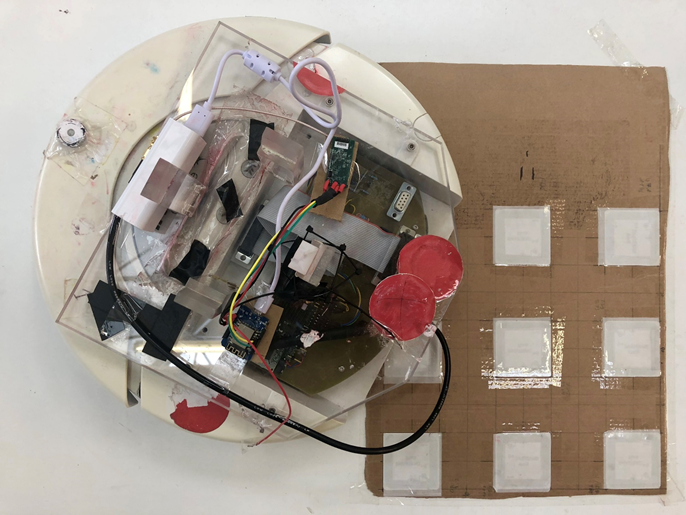
\includegraphics[width = 14cm]{Pictures/TestSetup}
\caption{testing setup for initialization procedure}
\label{TestSetup}
\end{figure}\\
The test platform was a field of 9 tags which were stuck on a piece of carton. The IDs and its positions are shown in tbl.\ref{IDs_Setup}.\\
\begin{table}[!htbp]
\begin{tabular}{|c|c|c|c|c|c|c|c|c|c|}
\hline
X-dir. [mm] & 0    & 100  & 200  & 0    & 100  & 200  & 0    & 100  & 200  \\ \hline
Y-dir. [mm] & 0    & 0    & 0    & 100  & 100  & 100  & 200  & 200  & 200  \\ \hline
ID tag [hex]    & AE4  & 689  & 47A  & 586  & 785  & ADC  & BF4  & 691  & 78D  \\ \hline
ID tag [dec]    & 2788 & 1673 & 1146 & 1414 & 1925 & 2780 & 3060 & 1681 & 1933 \\ \hline
\end{tabular}
\caption{Positions of the IDs in the test setup}
\label{IDs_Setup}
\end{table}\\
The reason for the small setup was the fact that until the end of the project only 10 tags were available. One of the following steps should be to extend the platform with more tags.\\
The initialization procedure was started via the GUI. A time value was added in the GUI to perform the 45$^\circ$ turns. This number was around 1125 ms and is highly correlated to the battery status of the AGV.\\

\subsection[Results]{Results\footnote{Stephan}}
A couple of tests on the test setup (previous section) were performed to compare the good results created with the simulated data with real measurements. The result of the position estimation was directly plotted in the console. The initial position was 200 mm in x- and y-direction and a varying orientation (0$^\circ$, 90$^\circ$, 180$^\circ$ and -90$^\circ$). Fig.\ref{ResultX} and fig.\ref{ResultY} illustrate the actual measurement results and the desired position in x- and y-direction. 
\begin{figure}[!htbp]
\centering
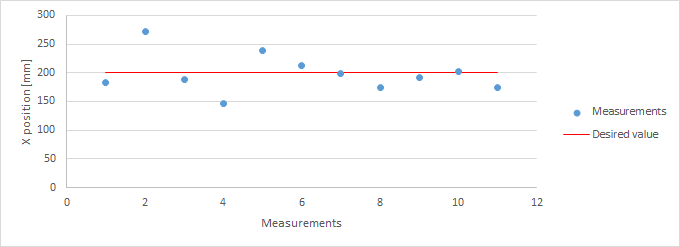
\includegraphics[width = 14cm]{Pictures/ResultX}
\caption{Estimated position in x-direction}
\label{ResultX}
\end{figure}\\
The average of the absolute error of the position in x-direction was 24.5 mm. The minimum and maximum error were 2 mm and 72 mm.\\
\begin{figure}[!htbp]
\centering
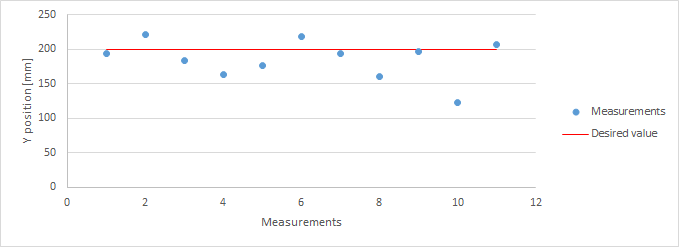
\includegraphics[width = 14cm]{Pictures/ResultY}
\caption{Estimated position in y-direction}
\label{ResultY}
\end{figure}\\
The average of the absolute error of the estimation of the position in y-direction is with 23.3 mm, a minimum error of 3 mm and an maximum error of 77 mm very similar to the results from the estimation of the x-direction. The computation of the overall error of the position has an average derivation of 37.5 mm and a minimum and maximum error of 6.3 mm and 77 mm.\\
\begin{figure}[!htbp]
\centering
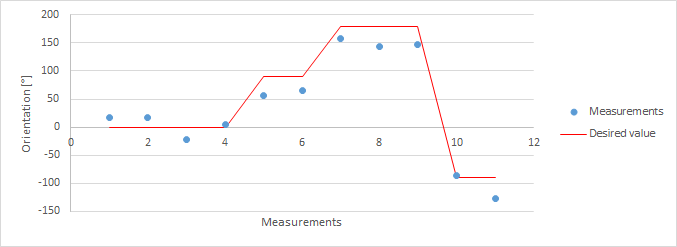
\includegraphics[width = 14cm]{Pictures/ResultO}
\caption{Estimated orientation}
\label{ResultO}
\end{figure}\\
For the estimation of the orientation, the average of the absolute error was 23$^\circ$ with a minimum and a maximum value of 3.9$^\circ$ and 37.5$^\circ$. The measurements also shows that an estimation of the position with a big error not necessarily leads to a big error in the estimation of the orientation (see measurement 4 in fig.\ref{ResultX},  \ref{ResultY} and \ref{ResultO}).\\
An extension of the results could also be an analyse of the estimated positions of the antenna at the measurement points. Those points were also plotted in the console. \\

%\subsection{Improvements}

